\section{Geração de solução final}
\label{geracao-solucao-final}

Após executar as etapas de verificação de custo para todos os índices candidatos gerados, a solução final é formada escolhendo-se os índices que apresentaram o menor custo para a execução das consultas, ao mesmo tempo em que podem ser aproveitados pela maior quantidade de consultas diferentes. Um fluxograma de como esse processo é realizado é apresentado na figura \ref{fig:escolha-solucao-final}.


\begin{figure}[!htb]
  \centering
  \caption{Fluxograma para escolha dos índices da solução final.}
  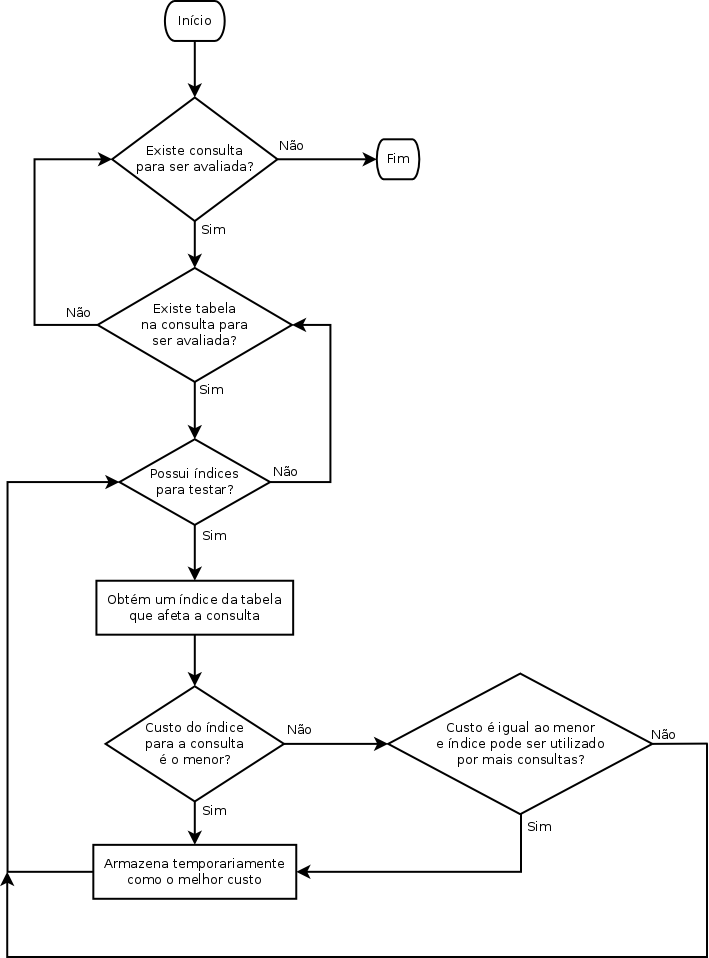
\includegraphics[width=\textwidth]{escolha-solucao-final.png}
  \fonte{Elaborado pelo autor.}
  \label{fig:escolha-solucao-final}
\end{figure}


O algoritmo de escolha dos índices para a solução final percorre todas as consultas que foram analisadas e, para cada tabela utilizada na consulta, escolhe o índice candidato com o menor custo. Em caso de dois ou mais índices oferecerem o mesmo custo, a ferramenta irá optar pelo índice que possa ser utilizado por mais consultas, eliminando a necessidade de índices adicionais e evitando que sejam escolhidos índices muito específicos.
